\section{Threat Model}
\label{Adversary Model}

We align our threat model with the same basic assumptions as described in~\cite{veen:typearmor} w.r.t. the forward-edge.
More precisely, we assume a resourceful attacker that has read and write access to the data 
sections of the attacked program binary. We assume that the protected binary does not contain 
self-modifying code, handcrafted assembly or any kind of obfuscation. We also consider pages 
to be either writable or executable but not both at the same time. Further, we assume 
that the attacker has the ability to exploit an existing memory corruption in order to hijack the program
control flow. 
We consider a powerful, yet realistic adversary
model that is consistent with previous work on code-reuse
attacks and mitigations \cite{volodymyr:cpi}. 
The adversary is aware of the
applied defenses and has access to the source and non-randomized 
binary of the target application.
We assume a powerful attacker which can exploit (bend)
any backward-edge based indirect program transfer and
has the capability to make arbitrary memory writes. 
We assume that other forward-edge and backward-edge protection mechanisms
can be used in parallel with our techniques.
These defense
mechanisms are orthogonal to our protection policies. Our
approach does not rely on information hiding from the
attacker and as such we can tolerate arbitrary reads. 
Finally, the analyzed program binary is not hand-crafted and the compiler which was used
to generate the program binary adheres to one of the 
following most used caller-callee calling conventions \cite{arm:abi, microsoft:abi, itanium:abi}.

\begin{center}
\begin{figure*}[t!]
\centering
   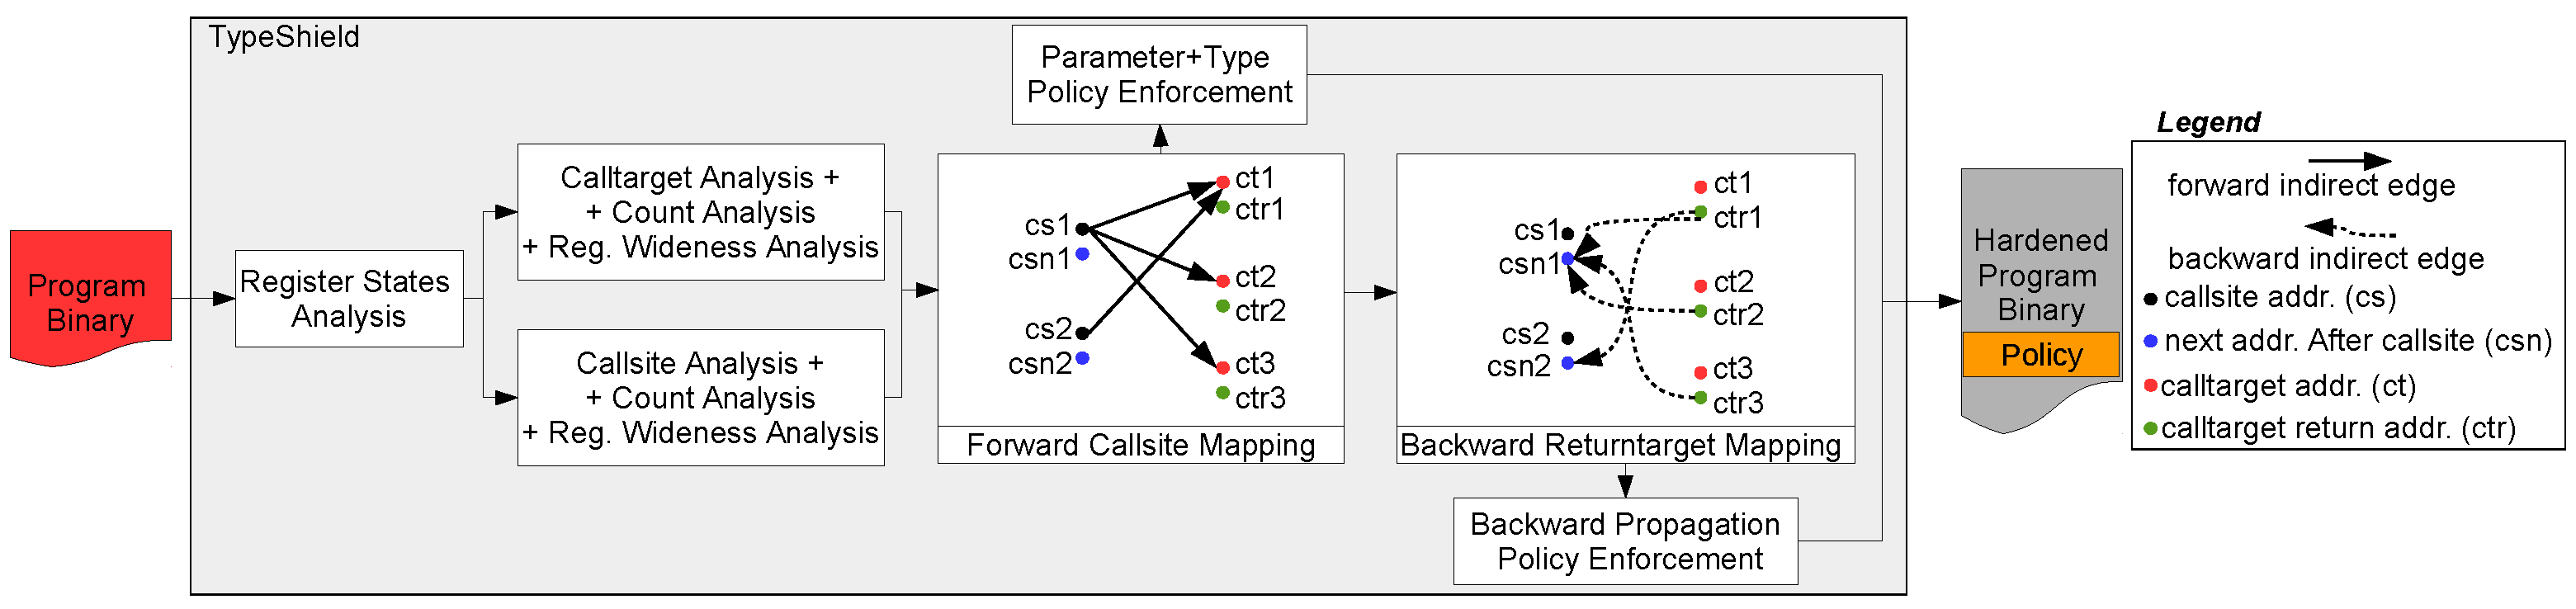
\includegraphics[width=.88\textwidth]{figures/overview.pdf}
    \caption{Overview of the main steps performed by \textsc{TypeShield} when hardening a program binary.}
    \label{System overview.}
    \vspace{-.5cm}
 \end{figure*}
\end{center}